\motto{As a practitioner, you want the simplest possible strategy; the one 
  that has the smallest amount of side effects; the minimum possible hidden complications \dots Your strategy to survive isn't 
  the same as ability to impress colleagues.}
\chapter{Practice}
\label{intro:03} % Always give a unique label
% use \chaptermark{}
% to alter or adjust the chapter heading in the running head

\abstract{In the previous chapter we discussed contracts at a very abstract level. Here we move from the previous abstract discussion
closer to the specific realization of those abstractions in the framework. 
}

\section{The Simplified Schema}
\label{sec:03:1}
\import{ch03/}{TheSimplifiedSchema.tex}

\section{Policies}
\label{sec:03:2}
Now that we have talked a bit about policies and modifications, below is a data structure overview of the same. The mathematical notation my not be
that familiar to you and if so don't be too put off. As with all mathematical notation in this book, there are comments to go with the notation
and the comments cover all of the important points. If you are interested you should be able to go from the comments to the notation and that
might be useful where you feel there are ambiguities. The mathematics is always correct and exists specifically to remove any ambiguity.

\import{ch03/}{Policy-sa.tex}

\section{Charges}
\label{sec:03:3}
There are currently five types of charges in the Socotra framework premiums (represented as PerilCharacteristics), taxes,
commissions, fees, and holdbacks. All these charges are represented by the same basic structure, a closed-open
interval, the data fields $[start\_timestamp, end\_timestamp)$, and a currency amount. It is
always assumed that $start\_timestamp \leq end\_timestamp$. Moreover if we have a description of the
policy coverage times as a set of intervals, then the range of a charge must always
fall inside the range of one of those intervals.
\begin{equation*}
\forall c \in Charge \cdot \exists i \in CoverageIntervals \cdot i.contains(c)
\end{equation*}
This requirement is not strictly required to bill properly but it is established behavior, that has a natural
interpretation. Every charge can be directly traced to a period of contracted coverage.

Amounts can have different interpretations depending on the type of charge and how it is calculated.
Premium amounts are always calculated from an original rate, usually in units of currency per month. Usually, then,
tax, commission, and rate fee amounts are calculated from the premium amounts by multiplying them by a percentage.
When the charges, above, are scaled to a new time period, the amount is converted back into
a rate with units of currency per time and multiplied by the new time period. It's a bit
round about and round trip conversion looses precision but that is the legacy process. Flat fee and holdback amounts are
not interpreted as being derived from a rate. As one might expect their amounts remain constant no
matter what their associated interval is and the associated interval just indicates over what period of coverage the
charge was assessed.

Since the charges associated with a policy change over time, all charges have additional structure to track their
change history. Premium, tax, commission, and holdbacks are all modeled as temporal objects containing the temporal
fields $issued\_timestamp$ and $replaced\_timestamp$.
More commonly, you may have seen these fields in other frameworks by the names $valid\_from$ and
$valid\_to$. This simple structure is used to record an audit history and allow easy determination of the
coverage at any time, t, with a filter of the form
\begin{equation*}
issued\_timestamp \leq t < (replaced\_timestamp || infinity)
\end{equation*}
The history of fees is recorded in a much less convenient form. Each fee is connected to a linear list of fee\_versions, where
the latest fee\_version describes the currently assessed charges. Needless to say, a fee must have at least one version.
To find the coverage at time, t, one has to calculate
\begin{equation*}
min \lbrace v \in Version : t < (v.replaced\_timestamp || infinity) \rbrace
\end{equation*}

\subsection{Fees in Detail}
To give a better feeling for fees and how they behave under modification to a policy consider the following
graphical descriptions.
\import{ch03/}{FeeBehavior.tex}
\newpage

Below is Socotra mathematical specification which details the maintenance of flat fees as modifications are applied to a
policy. The important points are captured in the comments.
\import{ch03/}{FeesFlatCtx1-sa.tex}
\import{ch03/}{FeesFlatMch1-sa.tex}

\subsection{Holdbacks in Detail}

\begin{figure}[ht]
  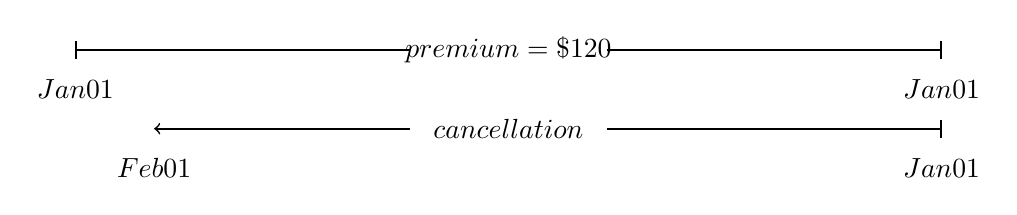
\begin{tikzpicture}
    \draw[|-,semithick] (0,-0.5) -- (4.25,-0.5);
    \draw (5.5, -0.5) node {$premium = \$120$};
    \draw[-|,semithick] (6.75,-0.5) -- (11,-0.5);
    \draw (0,-1) node {$Jan 01$};
    \draw (11,-1) node {$Jan 01$};
    
    \draw[<-,semithick] (1,-1.5) -- (4.25,-1.5);
    \draw (5.5, -1.5) node {$cancellation$};
    \draw[-|,semithick] (6.75,-1.5) -- (11,-1.5);
    \draw (1,-2) node {$Feb 01$};
    \draw (11,-2) node {$Jan 01$};
    
  \end{tikzpicture}   
  \caption{
    A policy and a cancellation
  }
  \label{ch03:fig:3:2}
\end{figure}

To explain holdbacks consider a policy running from Jan 1st of one year to Jan 1st of the next year, with a
premium of 120 dollars. If
a customer decided to cancel this policy starting at Feb 1st, then there are two adjustments that would
be made to this policy. First the premium would be prorated to account for the single month of coverage.
Assuming monthly proration 10 dollars would be charged for the month of coverage. Next there may be penalty
charges due to the customer canceling the policy early. We call these penalty charges holdbacks, and a typical
charge scenario, for our example, might be:
\begin{eqnarray*}
totalCharges_{Jan01->Feb01} & = & prorated(premium) + holdback \\
                          & = & (\frac{1}{12}) premium + 0.1(\frac{11}{12})(premium)
\end{eqnarray*}
where, here, the customer is charged a ten percent penalty fee on the part of the policy that was canceled.


Below is Socotra mathematical specification for maintaining holdbacks. The important points are captured in
the comments.
\import{ch03/}{ProrationCtx2-sa.tex}
\import{ch03/}{ProrationMch2-sa.tex}

\section{Observables}
\label{sec:03:4}

\import{ch03/}{CancellationCalculations-sa.tex}

\section{Modifications - The State Model}
\label{sec:03:5}
\import{ch03/}{TheBasicStateModel.tex}

\section{Characteristics - A Representative Interval}
\label{sec:03:6}

Characteristics are containers that record a set of attribute values
(ex: number\_of\_drivers = 2, make\_of\_car = Honda, resale\_value=10000)
which a policy contract is based on, and additionally a time interval over which
those attribute values are valid. Abstractly, it's a combination of a map and a time
interval. 

Below we just consider the time interval part of a characteristics and detail
how those intervals split as the standard modification operations are applied
to intervals
\import{ch03/}{CharacteristicsSplitCtx0-sa.tex}
\import{ch03/}{CharacteristicsSplitMch0-sa.tex}
